%%%%%%%%%%%%%%%%%%%%%%%%%%%%%%%%%%%%%%%%%%%%%%%%%%%%%%%%%%%%%%%%%%%%%%%%%%%%%%%%
% AMS Beamer series / Bologna FC / Template
% Andrea Omicini
% Alma Mater Studiorum - Università di Bologna
% mailto:andrea.omicini@unibo.it
%%%%%%%%%%%%%%%%%%%%%%%%%%%%%%%%%%%%%%%%%%%%%%%%%%%%%%%%%%%%%%%%%%%%%%%%%%%%%%%%
%\documentclass[handout]{beamer}\mode<handout>{\usetheme{default}}
%
\documentclass[presentation, 9pt]{beamer}\mode<presentation>{\usetheme{AMSBolognaFC}}
%\documentclass[handout]{beamer}\mode<handout>{\usetheme{AMSBolognaFC}}
%%%%%%%%%%%%%%%%%%%%%%%%%%%%%%%%%%%%%%%%%%%%%%%%%%%%%%%%%%%%%%%%%%%%%%%%%%%%%%%%
\usepackage[T1]{fontenc}
\usepackage{wasysym}
\usepackage{amsmath,blkarray}
\usepackage[minted,most]{tcolorbox}
\usepackage{centernot}
\usepackage{fontawesome}
\usepackage{fancyvrb}
\setminted[scala]{fontsize=\scriptsize,baselinestretch=1,obeytabs=true, tabsize=2}
\usepackage[ddmmyyyy]{datetime}
\renewcommand{\dateseparator}{}
%\renewcommand{\thefootnote}{\fnsymbol{footnote}}
\newcommand{\version}{1}
\usepackage[
	backend=biber,
	citestyle=authoryear-icomp,
	maxcitenames=1,
	bibstyle=numeric]{biblatex}

	\makeatletter

\addbibresource{biblio.bib}
%%%%%%%%%%%%%%%%%%%%%%%%%%%%%%%%%%%%%%%%%%%%%%%%%%%%%%%%%%%%%%%%%%%%%%%%%%%%%%%%
\title[Scala(e) to the large]
{Scala(e) to the large}
%
\subtitle[Concurrent programming in Scala and relevant Frameworks]
{Concurrent programming in Scala and relevant Frameworks}
%
\author[\sspeaker{Aguzzi}]
{\speaker{Gianluca Aguzzi} \href{mailto:gianluca.aguzzi@unibo.it}{gianluca.aguzzi@unibo.it}}
%
\institute[DISI, Univ.\ Bologna]
{Dipartimento di Informatica -- Scienza e Ingegneria (DISI)\\
\textsc{Alma Mater Studiorum} -- Universit{\`a} di Bologna \\[0.5cm]
\textbf{Talk @} \bold{Paradigmi di Progettazione e Sviluppo}}
%
\renewcommand{\dateseparator}{/}
\date[\today]{\today}
%
\AtBeginSection[]
{
  \begin{frame}
  \frametitle{Contents}
  \tableofcontents[currentsubsection, 
	sectionstyle=show/shaded, 
	subsectionstyle=show/shaded]
  \end{frame}
}
\AtBeginSubsection[]
{
  \begin{frame}
  \frametitle{Contents}
  \tableofcontents[currentsubsection, 
	sectionstyle=show/shaded, 
	subsectionstyle=show/shaded]
  \end{frame}
}
%%%%%%%%%%%%%%%%%%%%%%%%%%%%%%%%%%%%%%%%%%%%%%%%%%%%%%%%%%%%%%%%%%%%%%%%%%%%%%%%
\begin{document}
%%%%%%%%%%%%%%%%%%%%%%%%%%%%%%%%%%%%%%%%%%%%%%%%%%%%%%%%%%%%%%%%%%%%%%%%%%%%%%%%

%/////////
\frame{\titlepage}
%/////////

%===============================================================================
\section{Introduction}
\begin{frame}{Why Scala?}
	\begin{itemize}
		\item Several languages address concurrency by design (e.g. \emph{Erlang}, \emph{Go}, ...)
		\item Scala is used for several distributed \& concurrent computing frameworks
		\begin{itemize}
			\item Both in research (\bold{ScalaLoci}, \bold{ScaFi}) and in industry (\bold{Akka}, \bold{Spark}, \bold{Flink}) 
		\end{itemize}
  	\item Reasons:
    \begin{enumerate}
				\item Scala \emph{syntactic flexibility}: enable crafting of embedded domain-specific languages,
				with Scala serving as a host language, emulating several programming models (e.g., actor)
				\item Scala is a \emph{safe} language: static type safety reduces the amount of possible errors that developers have to care of
				\item \emph{Interoperability}: Scala programs can seamlessly use existing Java libraries, and interact with
				Java's rich ecosystem (recently with JS and Native too)
		\end{enumerate}
	\end{itemize}
	\begin{itemize}
		\item Today topics: 
		\begin{enumerate}
			\item Recall on low-level concurrency API (JVM model)
   		\item Future \& Promise as platform-independent concurrency mechanisms
     	\item Functional concurrency management: Monad effects (IO \& Task) and (Functional) Reactive streams 
      \item Application example leveraging Effects \& Functional Reactive Programming (FRP)
		\end{enumerate}
	\end{itemize}
	\begin{itemize}
		\item Code repositories:
		\begin{itemize}
			\item Examples of concurrency in Scala \href{https://github.com/cric96/scala-concurrent-programming}{\faLink}
   		\item FRP game \href{https://github.com/cric96/scala-frp-gui}{\faLink}
     	\item ``Monadic'' GUI \href{https://github.com/cric96/scala-functional-gui}{\faLink}  
		\end{itemize}
	\end{itemize}
\end{frame}
%===============================================================================
\section{Concurrency}
\subsection{Low-level API}
\begin{frame}[fragile, allowframebreaks]{JVM concurrency API in Scala}
	\begin{itemize}
		\item The low-level Scala API is similar to the JVM counterpart
  	\begin{alertblock}{Thread}
			Independent computations occurring in the same process 
			\begin{itemize}
				\item Creation \& starting of concurrent computation
    		\item[] \begin{tcolorbox}[left=0pt, top=0pt, bottom=0pt]
					\begin{minted}{scala}
val thread = Thread(() => println("Here")
//OOP style
class MyThread extends Thread:
  override def run: Unit = ...
thread.start() // side effect, the computation starts
					\end{minted}
				\end{tcolorbox}

				\item Explicit synchornization through \texttt{join}
				\item[] \begin{tcolorbox}[left=0pt, top=0pt, bottom=0pt]
					\begin{minted}{scala}
val threadA = ...
val threadB = ...
threadA.start()
threadA.join() // synchornization point, A andThen B
threadB.start()
					\end{minted}
				\end{tcolorbox}
			\end{itemize}
		\end{alertblock}
		\begin{alertblock}{Monitor}
			\begin{itemize}
				\item Ensure exclusive access to resources 
				\item Synchronizing and communicating among users
    		\item Implemented through \texttt{synchronized} (not a keyword!!), \texttt{wait}, \texttt{notify} and \texttt{notifyAll}
      	\item Or by using high-level API
    		\item[] \begin{tcolorbox}[left=0pt, top=0pt, bottom=0pt]
					\begin{minted}{scala}
trait Counter:
	def tick(): Unit
	def value: Int

object ThreadSafeCounter:
	def apply(): Counter = new Counter:
    private var count = 0 // encapsulated state
    // synchronized is not a keyword.. so you cannot write synchronized def tick ...
    def tick(): Unit = this.synchronized(count += 1)
    def value = this.synchronized(count)
					\end{minted}
				\end{tcolorbox}
			\end{itemize}
		\end{alertblock}
	\end{itemize}
\end{frame}
\begin{frame}{Considerations}
	\begin{itemize}
		\item Typically, \texttt{Thread} (and low-level APIs) are not used directly in Scala
  	\begin{itemize}
			\item \texttt{Thread}s computations do not \emph{compose} well (we will see what we mean with composition) \dots
   		\item \dots and Scala loves composition (e.g., for-comprehension)
     \item \texttt{Thread}s are not declarative (encapsulate the effect of computations)
		\end{itemize}
 		\item \texttt{scala.concurrent} exposes several high-level patterns to handle concurrency \& synchronization
 		\item JVM API cannot be used in different platforms (i.e., Scala.js)
   	\item Use this API when:
    \begin{itemize}
			\item You need to build very high-performant application
   		\item You create an application that targets only the JVM ecosystem 
		\end{itemize}
		\item in all the other cases, you should use \texttt{scala.concurrent} API
  \end{itemize}
\end{frame}
\begin{frame}[fragile, allowframebreaks]{Execution Context}
	\begin{itemize}
		\item An \texttt{ExecutionContext} can execute program logic asynchronously, typically but not necessarily on a thread pool.
		\item First layer of abstraction over \texttt{Thread}s used for large number of small concurrent tasks with high
		throughput,
  	\item Similar to the \texttt{Executors} Java framework, but platform-independent 
   	\item Drive to pass the context ``implictily'' (i.e., using \texttt{given} \& \texttt{using}) 
		 \item[] \begin{tcolorbox}[left=0pt, top=0pt, bottom=0pt]
			\begin{minted}{scala}
def sayGreet()(using context: ExecutionContext): Unit =
	context.execute(() => println("run!"))

@main def executeTask: Unit =
	val context = ExecutionContext.global // global execution context
	context.execute(() => println("Task done!"))
	val fromExecutors = ExecutionContext.fromExecutor(Executors.newSingleThreadExecutor())
	fromExecutors.execute(() => println("Java wrapper"))
	//sayGreet() // error
	given ExecutionContext = fromExecutors // enrich the context
	sayGreet()
			\end{minted}
		\end{tcolorbox}
	\end{itemize}
	\framebreak
	\begin{itemize}
		\item Used as a ``execution'' context platform for high level concurrent abstraction (e.g., Future)
  	\item We can built a ``context''-oriented DSL for async computation:
		\item[] \begin{tcolorbox}[left=0pt, top=0pt, bottom=0pt]
			\begin{minted}{scala}
/* In scala, a natural way to "enrich" the language consist in using contexts + entrypoints.*/
def async(any: => Unit)(using ExecutionContext): Unit =
	summon[ExecutionContext].execute(() => any)

@main def tryDsl(): Unit =
	given ExecutionContext = ExecutionContext.global // express the context ==> enrich the language
	println("Do somethings")
	async { // I can use async like a language API
		println("order??")
	}
	println("After")
			\end{minted}
		\end{tcolorbox}
	\end{itemize}
\end{frame}
\begin{frame}[fragile]{Parallell collections example: toward declative parallel computations}
	\begin{itemize}
		\item Scala collections can be transformed into their parallel counterparts by calling the par
		method (Scala < 2.13)
		\item It exists solely in order to improve the running time of the program
  	\item Idea: I express a data pipeline computation and then the runtime optimizes it using several cores
		\item[] \begin{tcolorbox}[left=0pt, top=0pt, bottom=0pt]
			\begin{minted}{scala}
(0 until 100000).par.map(_.toString).filter(x => x == x.reverse)
			\end{minted}
		\end{tcolorbox}
		\item Can I reach the same declarative approach for a general concurrent program? Yes, with \emph{Future} 
	\end{itemize}
\end{frame}
\subsection{Asynchronous Programming (scala.concurrent)}
\begin{frame}[fragile]{Future}
	\begin{alertblock}{Definition}
		\centering
		\begin{itemize}
			\item \emph{``A Future represents a value which may or may not currently be available, but will be available at some point, or as an exception if that value could not be made available.''}
		\end{itemize}
	\end{alertblock}
\begin{itemize}
 \item It is the idiomatic wat to express concurrent computations
 \item You handle the result of a future with \emph{callback} methods \emph{transformation} methods
 \item Future is a monad that models \emph{latency} as an \emph{effect}
 \item Futures are one-shot: the value contained by a future will be eventually available
 \item Futures are \emph{eager}: the computation starts on \texttt{Future} creation
 \item Futures \emph{memoize} the value: once the computation is over, the data will be always the same
 \item Examples: HTTP requests, File writing \& reading, TCP connections, ...
\end{itemize}
\begin{alertblock}{On notation}
	\begin{itemize}
		\item A \emph{future} value: \mintinline{scala}{trait Future[T]}
  	\item A future computation is an asynchronous computation that produces a future value: \mintinline{scala}{def something[T](...)(using ExecutionContext): Future[T]}
	\end{itemize}
\end{alertblock}
\end{frame}

\begin{frame}[fragile, allowframebreaks]{Future API}
	\begin{alertblock}{Future Creation}
 \begin{tcolorbox}[left=0pt, top=0pt, bottom=0pt]
				\begin{minted}{scala}
// To create a future computation, you have to enrich the context
using ExecutionContext = scala.concurrent.ExecutionContext.global
Future { 1 } // Future are eager, i.e., the computation starts on creation
val fututers = (1 to 10).map(Future.apply) // create sequence of future
Future.sequential(futures) // Map F[Future[_]] in Future[F[_]]
				\end{minted}
			\end{tcolorbox}
	\end{alertblock}
	\begin{alertblock}{Future Creation}
		\begin{tcolorbox}[left=0pt, top=0pt, bottom=0pt]
					 \begin{minted}{scala}
Future(10)
	.onComplete {
		case Success(value) => println(s"Hurra! $value")
		case Failure(exception) => println("Oh no..")
	}
					 \end{minted}
				 \end{tcolorbox}
		 \end{alertblock}
		 
\begin{alertblock}{Future Manipulation}
	\begin{tcolorbox}[left=0pt, top=0pt, bottom=0pt]
					\begin{minted}{scala}
val build = Future(Source.fromFile("build.sbt")) // Concurrent program expressed as sequence of map
	.map(source => source.getLines())
	.map(lines => lines.mkString("\n"))

val scalafmt = Future(Source.fromFile(".scalafmt.conf"))
	.map(source => source.getLines())
	.map(lines => lines.mkString("\n"))

// NB! scalafmt and build are concurrent here..
// Concurrent Program can be composed
val combine = build.flatMap(data => scalafmt.map(other => data + other)) 
					\end{minted}
				\end{tcolorbox}
\end{alertblock}
\begin{alertblock}{For Comprehension }
	\begin{tcolorbox}[left=0pt, top=0pt, bottom=0pt]
					\begin{minted}{scala}
def extractLines(source: Source): String = source.getLines().mkString("\n")
def readFile(name: String): Future[Source] = Future { Source.fromFile(name) }

val concurrentManipulation = for {
	buildSbt <- readFile("build.sbt")
	// synchornization point, scalafmt have to wait buildSbt future
	scalafmt <- readFile(".scalafmt.conf") // NB! build this two future are sequential
	fileSbt = extractLines(buildSbt) // I can you the data inside a Future manipulation..
	fileFmt = extractLines(scalafmt)
} yield (fileFmt + fileSbt)
					\end{minted}
				\end{tcolorbox}
\end{alertblock}
\begin{alertblock}{Context management}
		\begin{tcolorbox}[left=0pt, top=0pt, bottom=0pt]
						\begin{minted}{scala}
val myContext = ExecutionContext.fromExecutor(Executors.newSingleThreadExecutor())
def createFuture(using ExecutionContext) = Future {
	println(s"Hey! The thread is: ${Thread.currentThread().getName}")
}
createFuture(using global) // I can pass explicitly the context (i.e. when I want a fine control for execution)
given ExecutionContext = myContext // I can overwrite the execution context
createFuture
						\end{minted}
					\end{tcolorbox}
\end{alertblock}
\begin{alertblock}{Exception Management}
	\begin{tcolorbox}[left=0pt, top=0pt, bottom=0pt]
		\begin{minted}{scala}
val failed = Future.fromTry(Failure(new Exception("fail")))
failed.onComplete { case Failure(exception) =>
	println("error..")
}
// Special operator to wait a future.. Sync point (to avoid)
Await.ready(failed, Duration.Inf)
val fail = Future(1).failed // create a future that completes if the future fails
fail.foreach(println)
Await.ready(fail, Duration.Inf)
val empty = Future(1).filter(_ => false)
empty.failed.foreach(println) // failed
Await.ready(empty, Duration.Inf)
		\end{minted}
	\end{tcolorbox}
\end{alertblock}
\begin{alertblock}{Recover from Failure}
	\begin{tcolorbox}[left=0pt, top=0pt, bottom=0pt]
		\begin{minted}{scala}
val fail = Future("hello")
	.filter(_ == "ciao") // the future fail since "hello" != "ciao"
	.recoverWith(_ => Future("ciao")) // but I can recover it with another future (compose)
fail.foreach(println) // You can consume the future using foreach
		\end{minted}
	\end{tcolorbox}
\end{alertblock}
\begin{alertblock}{Blocking \& synchronization}
	\begin{tcolorbox}[left=0pt, top=0pt, bottom=0pt]
		\begin{minted}{scala}
val blocks = 20
val latch = CountDownLatch(blocks)
val all = (1 to blocks).map(i =>
	Future {
		println(s"Turn $i")
		blocking {
			latch.countDown()
			latch.await()
		}
	}
)

Await.ready(Future.sequence(all), Duration.Inf)
		\end{minted}
	\end{tcolorbox}
\end{alertblock}
\end{frame}

\begin{frame}[fragile]{Promise}
\begin{itemize}
	\item A Factory of \texttt{Future}
 	\item A \texttt{Promise} can be thought of as a writable, single-assignment container, which completes a future.
  \item \texttt{single-assignment} means that the \texttt{Promise} can be completed once (both with a value or with an exception)
  \item Use promises to bridge the gap between callback-based APIs and futures
  \item Use promises to extend futures with additional functional combinators. 
\end{itemize}
\begin{alertblock}{Promise API: in a nutshell}
	\begin{tcolorbox}[left=0pt, top=0pt, bottom=0pt]
		\begin{minted}{scala}
val promise = Promise[Int]() // Promise created..
promise.future.foreach(println) // "interface" to read the value
promise.success(10) // Everything ok!!
try promise.success(10) // Exception!!
catch case ex: IllegalStateException => println("Already completed!!")
		\end{minted}
	\end{tcolorbox}
\end{alertblock}
\end{frame}
\begin{frame}[fragile]{Future Consideration about FP}
\begin{itemize}
	\item Futures are \emph{eager} \faArrowRight \, we cannot express lazy computation
	\item[] 	\begin{tcolorbox}[left=0pt, top=0pt, bottom=0pt]
		\begin{minted}{scala}
Future { println("Start!!") } // the computation starts on creation
		\end{minted}
	\end{tcolorbox}
 	\item Futures are \emph{memoized} \faArrowRight \, we cannot restart a computation that brings this \texttt{Future} value
	 \item[] 	\begin{tcolorbox}[left=0pt, top=0pt, bottom=0pt]
		\begin{minted}{scala}
val result = Future { math.random }
result.foreach { println(_) }
result.foreach { pritnln(_) } // same result!
		\end{minted}
	\end{tcolorbox}
  \item Futures are not \emph{referential transparent} \faArrowRight \, we cannot build pure FP programs
	\item[] 	\begin{tcolorbox}[left=0pt, top=0pt, bottom=0pt]
		\begin{minted}{scala}
val random = Random(0)
def future(random: Random): Future[Int] = Future { random.nextInt(10) }
for {
	a <- future(random)
	b <- future(random)
} yield (a + b)
// !==
val futureRandom = future(Random(0))
for {
	a <- future(random)
	b <- future(random)
} yield (a + b)
		\end{minted}
	\end{tcolorbox}
	\item Futures combine the \emph{execution} and the \emph{computation} 
\end{itemize}
\end{frame}
\subsection{Task (IO) Monad}
\begin{frame}[fragile]{Effects (in FP)}
	\begin{itemize}
		\item An effect is a \emph{description} of an action (or actions) that will be taken when evaluation happens
		\item In Category Theory term, each Monad has an effect
		\begin{itemize}
			\item Option is a monad that models the effect of optionality (of being something optional)
   		\item Future is a monad that models the impact of latency
     	\item \texttt{IO} (in Cats ~\href{https://typelevel.org/cats/}{\faLink} term, \texttt{Task} in Monix \href{https://monix.io/}{\faLink}) is a monad that models the effect of \emph{computation}
		\end{itemize}
		\item Therefore, effects $\neq$ side-effects
		\begin{itemize}
			\item When a piece of code contains (express with effect) a side-effect, that action \emph{just happens}
		\end{itemize}
		\item \texttt{IO} (and \texttt{Task}, we will use this name hereafter) can be uxecuted asynchronously, in parallel, in different threads, ...
  	\item \bold{NB} When side-effecting code is wrapped in one \texttt{Task}...
		\begin{itemize}
			 \item the code itself still contains side-effects 
			 \item but we can reason about the whole thing as an effect, rather than as a side-effect
    \end{itemize}
		\item[] 	\begin{tcolorbox}[left=0pt, top=0pt, bottom=0pt]
			\begin{minted}{scala}
// this has a side-effect, but I can reason about this computation as Task[String]
Task { Source.fromFile(...) } 
			\end{minted}
		\end{tcolorbox}
		\item \bold{NB} \texttt{IO} is more general then \texttt{Task}, but today we consider these abstractions as the same
	\end{itemize}
\end{frame}
\begin{frame}{Task \href{https://monix.io/docs/current/eval/task.html}{\faLink}}
	\begin{alertblock}{Definition}
		Task represents a specification for a possibly lazy or asynchronous
computation, which when executed will produce a data as a result, along
with possible side effects.
	\end{alertblock}
	\begin{itemize}
  	\item doesn’t trigger the execution, or any effects 
		\begin{itemize}
			\item  Task does not represent a running computation or a value detached from time (like Future)
		\end{itemize}
   	\item allows for cancelling of a running computation
    \item \texttt{Task}s can be memoized (i.e., more control about the execution)
    \item it models a producer pushing only one value to one or multiple consumers
    \item \texttt{Task}s can express parallel computations
    \item It is referential transparent for most of the API, it contains unpure method marked with \mintinline{scala}{@UnsafeBecauseImpure}
    \begin{itemize}
			\item They should be used in the ``end-of-the-world'' (i.e., the main method)
		\end{itemize}
	\end{itemize}
\end{frame}
\begin{frame}[allowframebreaks, fragile]{Task API}
	\begin{alertblock}{Task Creation}
		\begin{tcolorbox}[left=0pt, top=0pt, bottom=0pt]
					 \begin{minted}{scala}
val now = Task.now {
	Math.random()
} // it evaluates the value asap and wraps it inside the task
//Task.apply =:= Task.eval
val standard = Task(Math.random()) // lazy.. the evaluation happen when the task is created
// Similar to a lazy val, the value it is evaluated once and then memoized (like future)
val once = Task.evalOnce {
	Math.random()
}
val future = Future(Math.random())
					 \end{minted}
				 \end{tcolorbox}
		 \end{alertblock}
		 \begin{alertblock}{Task Manipulation}
			\begin{tcolorbox}[left=0pt, top=0pt, bottom=0pt]
						 \begin{minted}{scala}
val file = Task(Source.fromFile("build.sbt"))
def linesFromSource(source: Source): Task[List[String]] = Task(source.getLines().toList).map(_.take(5))
// Sequence evaluation
val result = for {
	build <- file
	lines <- linesFromSource(build)
} yield lines.mkString("\n")
						 \end{minted}
					 \end{tcolorbox}
			 \end{alertblock}
			 \begin{alertblock}{Task Parallel Execution}
				\begin{tcolorbox}[left=0pt, top=0pt, bottom=0pt]
							 \begin{minted}{scala}
given Scheduler = monix.execution.Scheduler.Implicits.global
// Combine task to express parallel evaluation
// foreach run the execution (it needs the Scheduler)
for _ <- Task.parZip3(wait, wait, wait) do println("Parallel."))
Task
	.sequence(wait :: wait :: wait :: Nil)
	.foreach(_ => println("sequential..."))
Task
	.parSequence(wait :: wait :: wait :: Nil)
	.foreach(_ => println("parallel.."))
							 \end{minted}
						 \end{tcolorbox}
				 \end{alertblock}
				 \begin{alertblock}{Task Memoization}
					\begin{tcolorbox}[left=0pt, top=0pt, bottom=0pt]
								 \begin{minted}{scala}
// This data expresses a computation that produces a random value
val random = Task.eval(Math.random())
// This data expresses a computation that produces the same random value
val memo = random.memoize
								 \end{minted}
							 \end{tcolorbox}
					 \end{alertblock}
					 \begin{alertblock}{Task synchornization}
						\begin{tcolorbox}[left=0pt, top=0pt, bottom=0pt]
									 \begin{minted}{scala}
val semaphore = Semaphore[Task](1) // like a Lock
var shared = 0 // Just an example, in effect you should not use vars.. consider a shared resources..
def effect: Task[Unit] = Task {
	shared += 1
	println(Thread.currentThread().getName)
}
val syncComputation = for {
	synch <- semaphore
	tasks = (1 to 1000).map(_ => synch.withPermit(effect))
	par <- Task.parSequence(tasks)
} yield par

syncComputation.runSyncUnsafe()
assert(shared == 1000)
									 \end{minted}
								 \end{tcolorbox}
						 \end{alertblock}
\begin{alertblock}{Task error management}
	\begin{tcolorbox}[left=0pt, top=0pt, bottom=0pt]
										 \begin{minted}{scala}
// Tasks can fail...
val fail = Task.raiseError(new IllegalStateException("..."))
// I can handle error like Future (but with more flexibility, e.g., restarting the computation)
val recovered = fail.onErrorHandle(_ => 10)
										 \end{minted}
									 \end{tcolorbox}
							 \end{alertblock}
\begin{alertblock}{An Entire application expressed with Task}
	\begin{tcolorbox}[left=0pt, top=0pt, bottom=0pt]
					\begin{minted}{scala}
enum State:
	case Continue, End
val input = Task.eval(StdIn.readLine())
val hello = Task.evalOnce(println("Hello!! welcome to this beautiful game!!"))
lazy val parse: Task[Int] = input
	.map(_.toInt)
	.onErrorHandleWith(_ =>
		Task(println("Insert a number!!"))
			.flatMap(_ => parse)
	)
val toGuess = Task.evalOnce(Random.nextInt(10))
val toHigh = Task(println("The number is wrong!! (high)")).map(_ => State.Continue)
val toLow = Task(println("The number is wrong!! (low)")).map(_ => State.Continue)
val correct = Task(println("You won!!")).map(_ => State.End)

// The main, a typical way to express IO in functional program, through flatmap operations..
val game = for {
	_ <- hello
	number <- toGuess
	user <- parse
	state <-
		if (user < number) toLow else if (user > number) toHigh else correct
} yield state
					\end{minted}
				\end{tcolorbox}
		\end{alertblock}
\end{frame}
\subsection{Observable (Functional Reactive Programming)}
\begin{frame}{Observable \href{https://monix.io/docs/current/reactive/observable.html}{\faLink}}
% Please add the following required packages to your document preamble:
% \usepackage[table,xcdraw]{xcolor}
% If you use beamer only pass "xcolor=table" option, i.e. \documentclass[xcolor=table]{beamer}

	\begin{alertblock}{Definition}
		The Observable is a data type for modeling and processing asynchronous and reactive streaming of (possibly infinite) events with non-blocking back-pressure.
	\end{alertblock}
	\begin{itemize}
		\item At its simplest, an\ \texttt{Observable} is a replacement for your regular \texttt{Iterable} or Scala \texttt{Stream}, but with the ability to process asynchronous events without blocking.
  	\item Enables Functional Reactive Programming (FRP) 
   \item basically the Observer pattern on steroids
   \item Expresses lazy computations
   \item Inspired by ReacitveX \href{https://reactivex.io/intro.html}{\faLink}
	\end{itemize}
	\begin{alertblock}{Observable vs. Task}
		\begin{table}[]
			\centering
			\begin{tabular}{|c|c|c|}
			\hline
									 & \textbf{Single}                      & \textbf{Multiple}          \\ \hline
			\textbf{Synchronous}  & A                           & Iterable{[}A{]}   \\ \hline
			\textbf{Asynchronous} & Future{[}A{]} / Task{[}A{]} & Observable{[}A{]} \\ \hline
			\end{tabular}
			\end{table}
	\end{alertblock}
\end{frame}
\begin{frame}[fragile, allowframebreaks]{Observable API}
	\begin{alertblock}{Observable Creation}
		\begin{tcolorbox}[left=0pt, top=0pt, bottom=0pt]
					 \begin{minted}{scala}
val single = Observable.pure { println("hey!"); 10 } // print hey! because the value is evaluated asap
val delay = Observable.delay { println("hey"); 10 } // hey is printed each time the observable is consumed
// hey is printed once, then the value is memoized
val lazyObservable = Observable.evalOnce { println("hey"); 10 } 
val sideEffects = Observable.suspend {
	val effect = Source.fromFile("build.sbt")
	Observable.fromIterator(Task(effect.getLines()))
}
Thread.sleep(500)
					 \end{minted}
				 \end{tcolorbox}
		 \end{alertblock}	

		 \begin{alertblock}{Observable Composition (Sequential)}
			\begin{tcolorbox}[left=0pt, top=0pt, bottom=0pt]
						 \begin{minted}{scala}
// I can express infinite computation...
val stepper = Observable.fromIterable(LazyList.continually(10)).delayOnNext(500 milliseconds)
val greeter = Observable.repeatEval("Hello!!").delayOnNext(100 milliseconds)
val combined = for { // I can combine observable like list, option,....
	number <- stepper
	greet <- greeter
} yield (number, greet)
combined.foreach(println(_))
						 \end{minted}
					 \end{tcolorbox}
			 \end{alertblock}	

			 \begin{alertblock}{Observable Facade from other libraries}
				\begin{tcolorbox}[left=0pt, top=0pt, bottom=0pt]
							 \begin{minted}{scala}
val button = JButton("Click me!!")
// Using create api
val buttonObservable = Observable.create[Long](OverflowStrategy.Unbounded) { subject =>
	button.addActionListener((e: ActionEvent) => subject.onNext(e.getWhen))
	Cancelable.empty
}
// Or through subjects (i.e., tuple of observer and observable)
val subject = ConcurrentSubject[Long](MulticastStrategy.replay)
button.addActionListener((e: ActionEvent) => subject.onNext(e.getWhen))
							 \end{minted}
						 \end{tcolorbox}
				 \end{alertblock}	

				 \begin{alertblock}{Observables Backpressure}
					\begin{tcolorbox}[left=0pt, top=0pt, bottom=0pt]
								 \begin{minted}{scala}
val obs = Observable("A", "B", "C", "D", "E", "F", "G")
val syncObs = obs // By default, the obs manipulation are sequential
	.mapEval(elem => Task { println(s"Processing (1) : $elem"); elem + elem })
	.asyncBoundary(OverflowStrategy.Unbounded) // change the observable evaluation to another execution logic
	.mapEval(elem => Task { println(s"Processing (2) : $elem"); elem }.delayExecution(200 milliseconds))
								 \end{minted}
							 \end{tcolorbox}
					 \end{alertblock}	
					 \begin{alertblock}{Observables Parallell (similar to par)}
					\begin{tcolorbox}[left=0pt, top=0pt, bottom=0pt]
						\begin{minted}{scala}
val element = Observable.fromIterable((0 to 10))
val parallelMap = element.mapParallelOrdered(8)(elem =>
	Task(elem * 5).tapEval(id => Task(println(id + " " + Thread.currentThread().getName)))
)
val parallelUnorderedMap = element.mapParallelUnordered(8)(elem =>
	Task(elem * 5).tapEval(id => Task(println(id + " " + Thread.currentThread().getName)))
)
val mergeParallel = element.delayOnNext(100 milliseconds).mergeMap(_ => Observable(1).delayOnNext(100 milliseconds))
							\end{minted}
						\end{tcolorbox}
					\end{alertblock}	
					\begin{alertblock}{The Observable API is very Rich}
						\begin{itemize}
							\item Scala Doc \href{https://monix.io/api/current/monix/reactive/index.htmlhttps://monix.io/api/current/monix/reactive/index.html}{\faLink}
       				\item Documentation  \href{https://monix.io/docs/current/reactive/observable.html}{\faLink}
           \item Code example repository (about buffering, error handling, rate emission)  \href{}{\faLink}
						\end{itemize}
					\end{alertblock}	
\end{frame}
\begin{frame}[allowframebreaks, fragile]{FRP Application: A tentative design \href{https://github.com/cric96/scala-frp-gui}{\faLink}}
	\begin{itemize}
		\item The model is described using Algebraic Data Type and functional manipulation
		\item Rendering is wrapped on a \texttt{Task} (it expresses a side-effect)
  	\item The events (e.g., input from View, time evolution) are expressed as an \texttt{Observable}
   	\item The Model data evolve following the event \texttt{Observable} (creating an \texttt{Observable} of models)
    \item On top of Model \texttt{Observable}, the rendering Task is triggered (e.g. for each new Model data)
		\item \textbf{Potential benefits}
		\begin{itemize}
			\item Clean model as an immutable data (the manipulation is typically performed with \bold{lens}\href{https://www.optics.dev/Monocle/}{\faLink} \,)
   		\item Model evolution expressed as a composition between Tasks  
			\item Simplifies the interaction between View and Model (i.e., the Controller)
   		\item Side effects happen only at the end of the world
		\end{itemize}
	\end{itemize}
	\begin{alertblock}{UI (defines Input and Output boundary interface)}
	\begin{tcolorbox}[left=0pt, top=0pt, bottom=0pt]
		\begin{minted}{scala}
// a general UI: trait UI[Event, Data] ==> it contains side effects!! 
//(but they are wrapper with monadic abstractions)
// even more general: UI[Event, Data, F[_], R[_]]
trait UI:
	// Event source produced by this UI (outside of "functional" world, unsafe, unpure)
	def events: Observable[Event]
	// Render the world representation. It is an effect, therefore it returns a Task
	def render(world: World): Task[Unit]
		\end{minted}
		\end{tcolorbox}
	\end{alertblock}
	\begin{alertblock}{Model: set of data that expresses a snapshot of the "world"}
		\begin{tcolorbox}[left=0pt, top=0pt, bottom=0pt]
			\begin{minted}{scala}
enum Entity(...):
	case Player(...),

case class World(...)
			\end{minted}
			\end{tcolorbox}
		\end{alertblock}

		\begin{alertblock}{Update: namely how world should change}
			\begin{tcolorbox}[left=0pt, top=0pt, bottom=0pt]
				\begin{minted}{scala}
// This should be expressed as a function, (event, world) => Task[(Ager, Control)]
// Or Controller[E, M, F[_]] => (E, M) => F[(M, Control[E, M, F])]
trait Update extends ((Event, World) => Task[(World, Update)]):
	def andThen(control: Update): Update = ...

// We cannot use type because it became a cyclic reference
object Update:
	extension (function: (Event, World) => (World, Update))
		def lift: Update = ..
	// Creation API
	def same(function: (Event, World) => World): Update = ...

	def on[E <: Event](control: (E, World) => Task[World])(using ev: ClassTag[E]): Update = ...

	def combineTwo(engineA: Update, engineB: Update): Update = ...
		yield (lastWorld, combineTwo(newEngineA, newEngineB))

	def combine(engines: Update*): Update = ...
				\end{minted}
				\end{tcolorbox}
			\end{alertblock}

			\begin{alertblock}{Main Loop}
				\begin{tcolorbox}[left=0pt, top=0pt, bottom=0pt]
					\begin{minted}{scala}
def start(ui: UI): Task[Unit] =
	val time: Observable[Event] = TimeFlow // time progression (each 33 milliseconds)
    .tickEach(33 milliseconds).map(_.toDouble).map(Event.TimePassed.apply)
	val world = World.empty // Initial condition of the game
	val controls: Update = ... // set of controls that update the world state
	// Initial "loop" condition, update and world can evolte with events
	val init = Task((world, controls))
	val events =
		Observable(time, ui.events.throttleLast(33 milliseconds)).merge
	
	events
		// World evolve following the event 
		.scanEval(init) { case ((world, controls), event) => controls(event, world) }
		.doOnNext { case (world, _) => ui.render(world) } // For each frame, a rendering is requested
		.completedL // Compute until the game is over

					\end{minted}
					\end{tcolorbox}
				\end{alertblock}	
				\begin{alertblock}{Monadic "GUI"}

the curious can check the seminar of the past year, where I try to define GUI through monads with a similar design \href{https://github.com/cric96/MVC-meets-monad/releases/tag/0.1.0-2021-06-04T085146}{\faLink}
				\end{alertblock}
\end{frame}
\begin{frame}[fragile]{In Summary}
	\begin{itemize}
		\item Use Task to express any potential computation
  	\item Use Future to run a computation expressed through Task 
   	\item Use Observable \& Subject to express computation with multiple values (e.g. event sources)
    \item In this way:
    \begin{itemize}
			\item Your application becomes ``reactive''
   		\item Side effects happen only at the ``end-of-the-world''
     \item You can reason about effects, avoiding to care about side effects
     \item Error handling cames for free
     \item Your application works seamlessly in JVM \& JS world
		\end{itemize}
	\end{itemize}
	\begin{alertblock}{Final remark}
		\begin{columns}
			\begin{column}[c]{0.4\textwidth}
				``The IO monad does not make a function pure. It just makes it obvious that it's impure''
				\emph{Martin Odersky}
			\end{column}
			\begin{column}[c]{0.4\textwidth}

	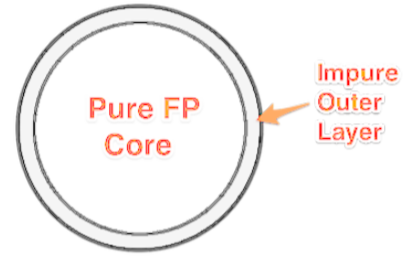
\includegraphics[width=4cm]{img/pure-impure.png}
			\end{column}
		\end{columns}
	\end{alertblock}
\end{frame}
\section{Frameworks}
\begin{frame}{Scala: Best choice to create complex \& distributed Framework}
	\begin{itemize}
		\item DSL hides complexity giving high-level API
  	\item Contextual information (i.e. to use API) is passed through \emph{implicit/given} giving the impression of "enrich" the language
   \item Strong type system enforces compile-time correctness
   \item Programmers focus on the intent (declarative approach)
   \item Future / Observable / Task example:
   \begin{itemize}
			\item Intent: express possibly concurrent computations;
   		\item DSL: monadic manipulation, how the data should be combined \& transformed
     \item Context: ExecutionContext, where the computation will be executed 
	 \end{itemize}
	 \item In the next slides:
	 \begin{itemize}
			\item two relevant examples of industry-proven scala framework (Akka \& Spark)
   	\	\item two examples of reasearch oriented libraries \& framework (ScaFi \& ScalaLoci) 
	 \end{itemize}
	\end{itemize}
\end{frame}
\subsection{Industry-ready}
\begin{frame}[c]{The Akka actor toolkit}
%/////////
Akka is a toolkit for building highly concurrent, distributed, and resilient
message-driven applications for Java and Scala
\begin{itemize}
	\item It is \bold{the} implementation of the Actor model on the JVM
	\item It extends the basic Actor model with more convenient \& advanced features
	\item Akka supports and integrates into an ecosystem of tools for distributed systems
 \begin{itemize}
		\item Play (web framework), Spray (REST), Lagom (microservices), Apache Flink (stream/batch
		processing), Gatling (load-testing)...
		\item Actors as a basic building block
 \end{itemize}
 \item Production-proved: \url{https://www.lightbend.com/case-studies}
 \item \bold{Website}: \url{https://akka.io/}
 \item \bold{Docs}: \url{https://akka.io/docs/}
\end{itemize}
\begin{alertblock}{Akka APIs and DSLs \href{https://doc.akka.io/docs/akka/current/typed/from-classic.html}{\faLink}}
	\begin{itemize}
		\item Akka provides APIs for developing actor-based systems with Java and Scala DSLs
		\item \emph{Akka Typed}: new, type-safe API
		\item \emph{Akka Classic}: original API (still fully supported)
		\item These may coexist in a single application
	\end{itemize}
\end{alertblock}
\end{frame}

\begin{frame}{Spark}
	\begin{itemize}
		\item Apache Spark is a unified analytics engine for large-scale data processing.
		\begin{itemize}
			\item It provides high-level APIs in Java, Scala, Python
		\end{itemize}
		\item Dataset as a primary abstraction that consists of a distributed collection of items 
  	\item \textbf{The} framework for big data management.
   \item Data processing executed on \emph{cluster}
   	\item It also supports a rich set of higher-level tools including 
		 \begin{itemize}
			\item Spark SQL for SQL and structured data processing, 
   		\item MLlib for machine learning,  
		 \end{itemize}
	\end{itemize}
	\centering
	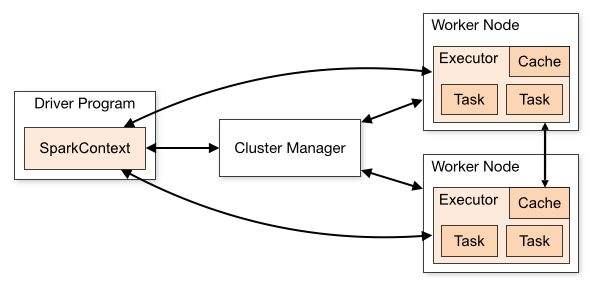
\includegraphics[width=5cm]{img/cluster-overview.png}
\end{frame}
\begin{frame}[fragile]{Spark -- Example}
	\begin{alertblock}{}
		\begin{tcolorbox}[left=0pt, top=0pt, bottom=0pt]
			\begin{minted}{scala}
// Context
lazy implicit val spark =
	SparkSession.builder()
		.master("local")
		.appName("spark_test")
		.getOrCreate()

import spark.implicits._ // Required to call the .toDF function later
val html = scala.io.Source
	.fromURL("http://files.grouplens.org/datasets/movielens/ml-100k/u.data")
	.mkString // Get all rows as one string
val seqOfRecords = ...
// Give whatever column names you want
val df = seqOfRecords.toDF("userID", "movieID", "ratings", "timestamp")
// Data manipulation (I do not care where this will be executre)
df
	.select("ratings") // select the "ratings row"
	.groupBy("ratings") // group by on ratings
	.count // count the total number of row for each rating
	.sort(col("count").desc) // sort the ratings using the count
	.show()
			\end{minted}
		\end{tcolorbox}
	\end{alertblock}
\end{frame}
\subsection{Research Framework}
\begin{frame}{ScaFi (Scala Fields)}
\begin{itemize}
	\item ScaFi (Scala Fields) is a Scala-based library and framework for \bold{Aggregate Programming}.
	\begin{itemize}
		\item A macro-programming approach to program large-scale distriubted system, formally grounded in Field Calculus
	\end{itemize}
	\item \textbf{Goal}: programming the collective behaviour of \emph{aggregates} of devices
 	\item Provides a DSL and API for writing, testing, and running aggregate programs
  \item ScaFi-Web: A web playground based on ScaFi \href{https://scafi.github.io/web/}{\faLink}
	\item ScaFI is a \emph{multi-module} and \emph{cross platform} scala project:
	\begin{itemize}
		\item \texttt{\bold{scafi-commons}} | provides basic abstractions and utilities (e.g., spatial and temporal abstractions);
		\item \texttt{\bold{scafi-core}} | represents the core of the project and provides an aggregate programming DSL (syntax, semantics, and a virtual machine for evaluation of programs), together with a ``standard library'' of reusable functions;
		\item \texttt{\bold{scafi-simulator}}: provides a basic support for simulating aggregate systems;
		\item \texttt{scafi-simulator-gui} | provides a GUI for visualising and interacting with simulations of aggregate systems;
		\item \texttt{spala} (``spatial Scala''---i.e., a general Aggregate Computing platform | provides an actor-based aggregate computing middleware;
		\item \texttt{scafi-distributed} |  ScaFi integration-layer for \texttt{spala}, which can be leveraged to set up actor-based deployments of ScaFi-programmed systems.
		\end{itemize}
\end{itemize}


\end{frame}
\begin{frame}{ScaFi (Scala Fields) -- Architecture}
	\centering
	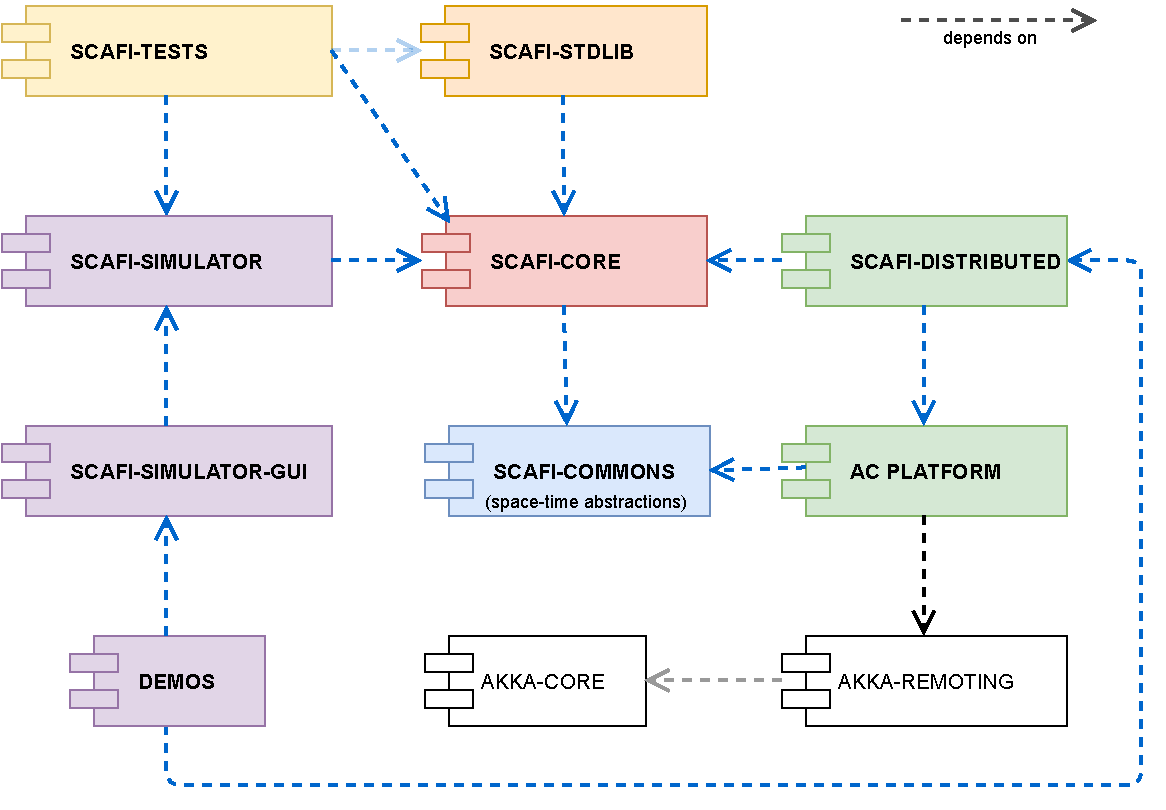
\includegraphics[width=10cm]{img/scafi-project-org.pdf}
\end{frame}
\begin{frame}[fragile, allowframebreaks]{ScaFi (Scala Fields) -- Usage example \href{https://github.com/cric96/spark-mini-example}{\faLink}}
	\begin{alertblock}{Distributed sensing}
		\begin{tcolorbox}[left=0pt, top=0pt, bottom=0pt]
			\begin{minted}{scala}
// Incarnation: the context of an aggregate program
import it.unibo.scafi.incarnations.BasicSimulationIncarnation.*
class DistributedTemperatureSensing extends AggregateProgram
	// Libraries, expressed as mix-in
	with BlockG with BlockC with BlockS with BlocksWithGC with StandardSensors { 
	// "entry point", kind of "end-of-the-world" of effects
	override def main: Double = {
		val area = 50 // area size in which I want sense temperature
		val leader = S(area, nbrRange) // center of that area
		val potential = distanceTo(leader) // used to send information to leader
		val areaTemperature = average(leader, temperature) // average temperature value
		broadcast(leader, areaTemperature) // share the temperature to devices
	}
	def temperature: Double = randomGenerator().nextDouble() * 10 + 20
}
val program = new DistributedTemperatureSensing
			\end{minted}
		\end{tcolorbox}
	\end{alertblock}
\centering
	\begin{alertblock}{Self-healing channel}
		\begin{tcolorbox}[left=0pt, top=0pt, bottom=0pt]
			\begin{minted}{scala}
class Channel extends AggregateProgram 
	with StandardSensors with BlockG {
	override def main() = {
		def source : Boolean = sense("source") // zone of the space that we want to link to target
		def target : Boolean = sense("target") // the target of the channel
		def channel(source: Boolean, target: Boolean, width: Double): Boolean = {
			// All nodes that are inside the channel
			distanceTo(source) + distanceTo(target) <= distanceBetween(source, target) + width
		}
		val channelWidth = 1
		channel(source, target, channelWidth)
	}
}
			\end{minted}
		\end{tcolorbox}
	\end{alertblock}
\framebreak
\begin{columns}
	\begin{column}[c]{0.4\textwidth}
		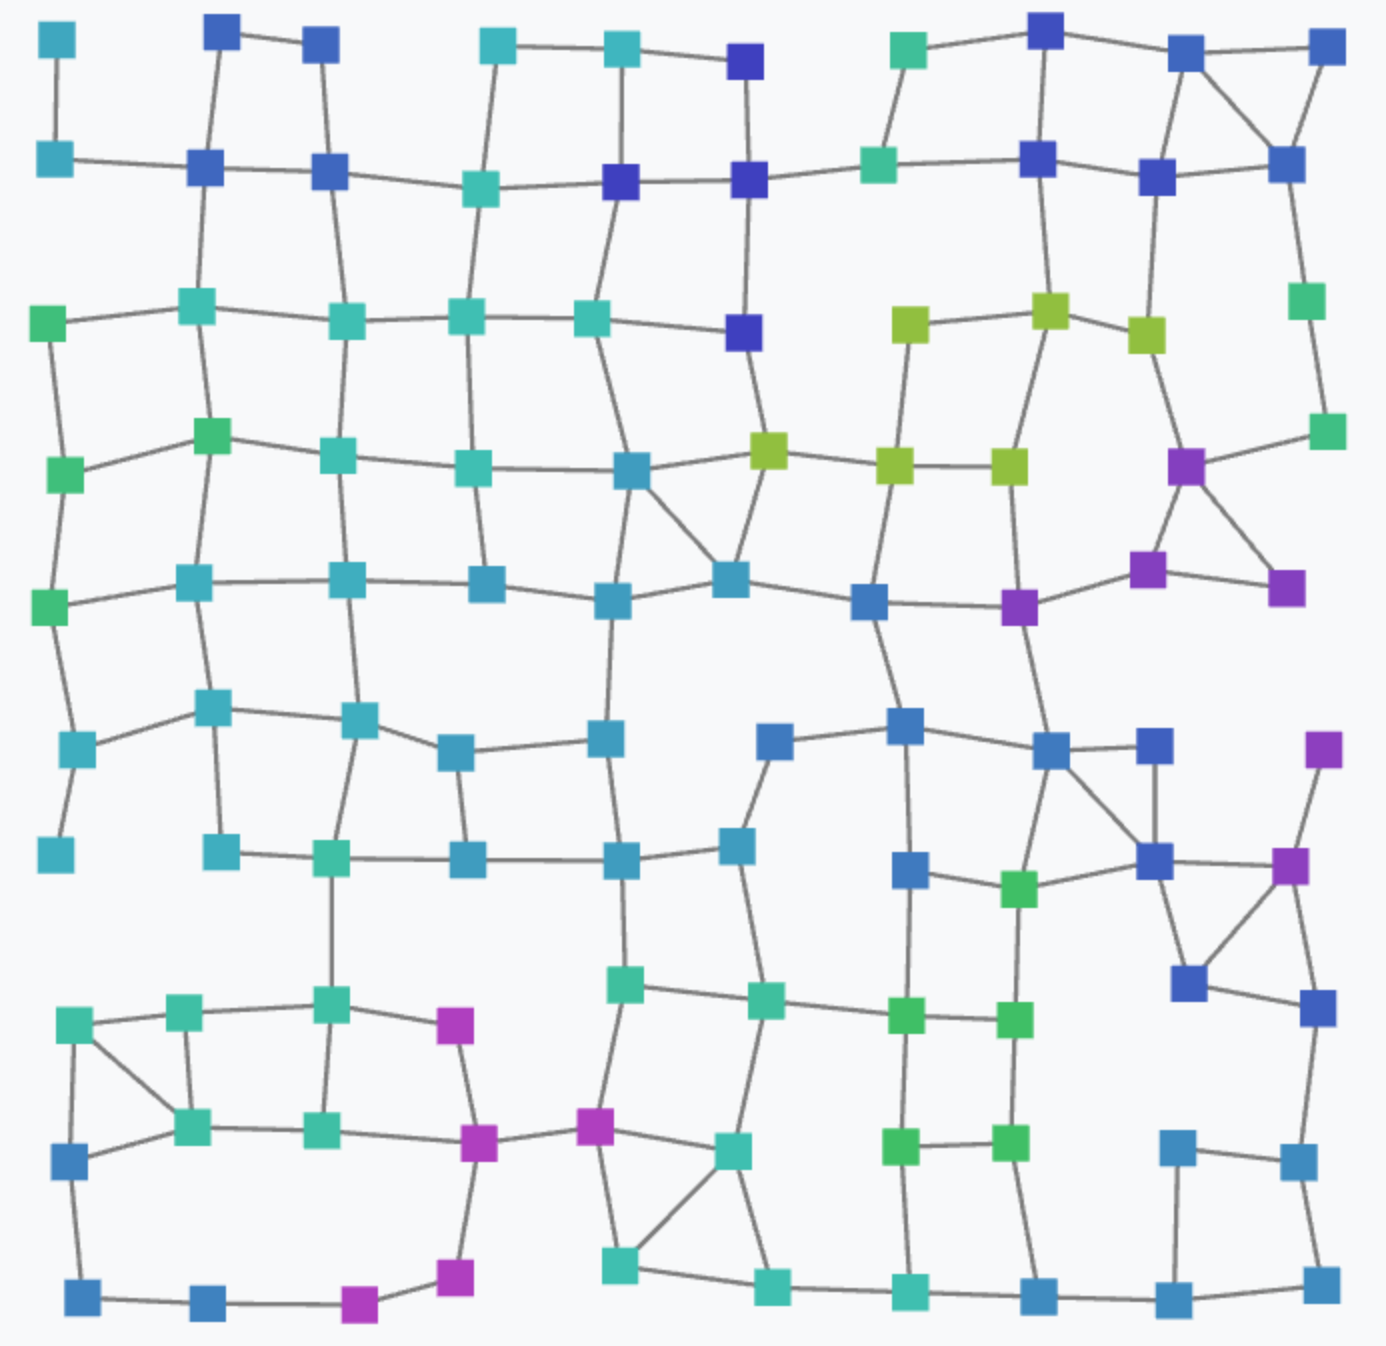
\includegraphics[width=5cm]{img/temperature.png}
	\end{column}
	\begin{column}[c]{0.4\textwidth}
		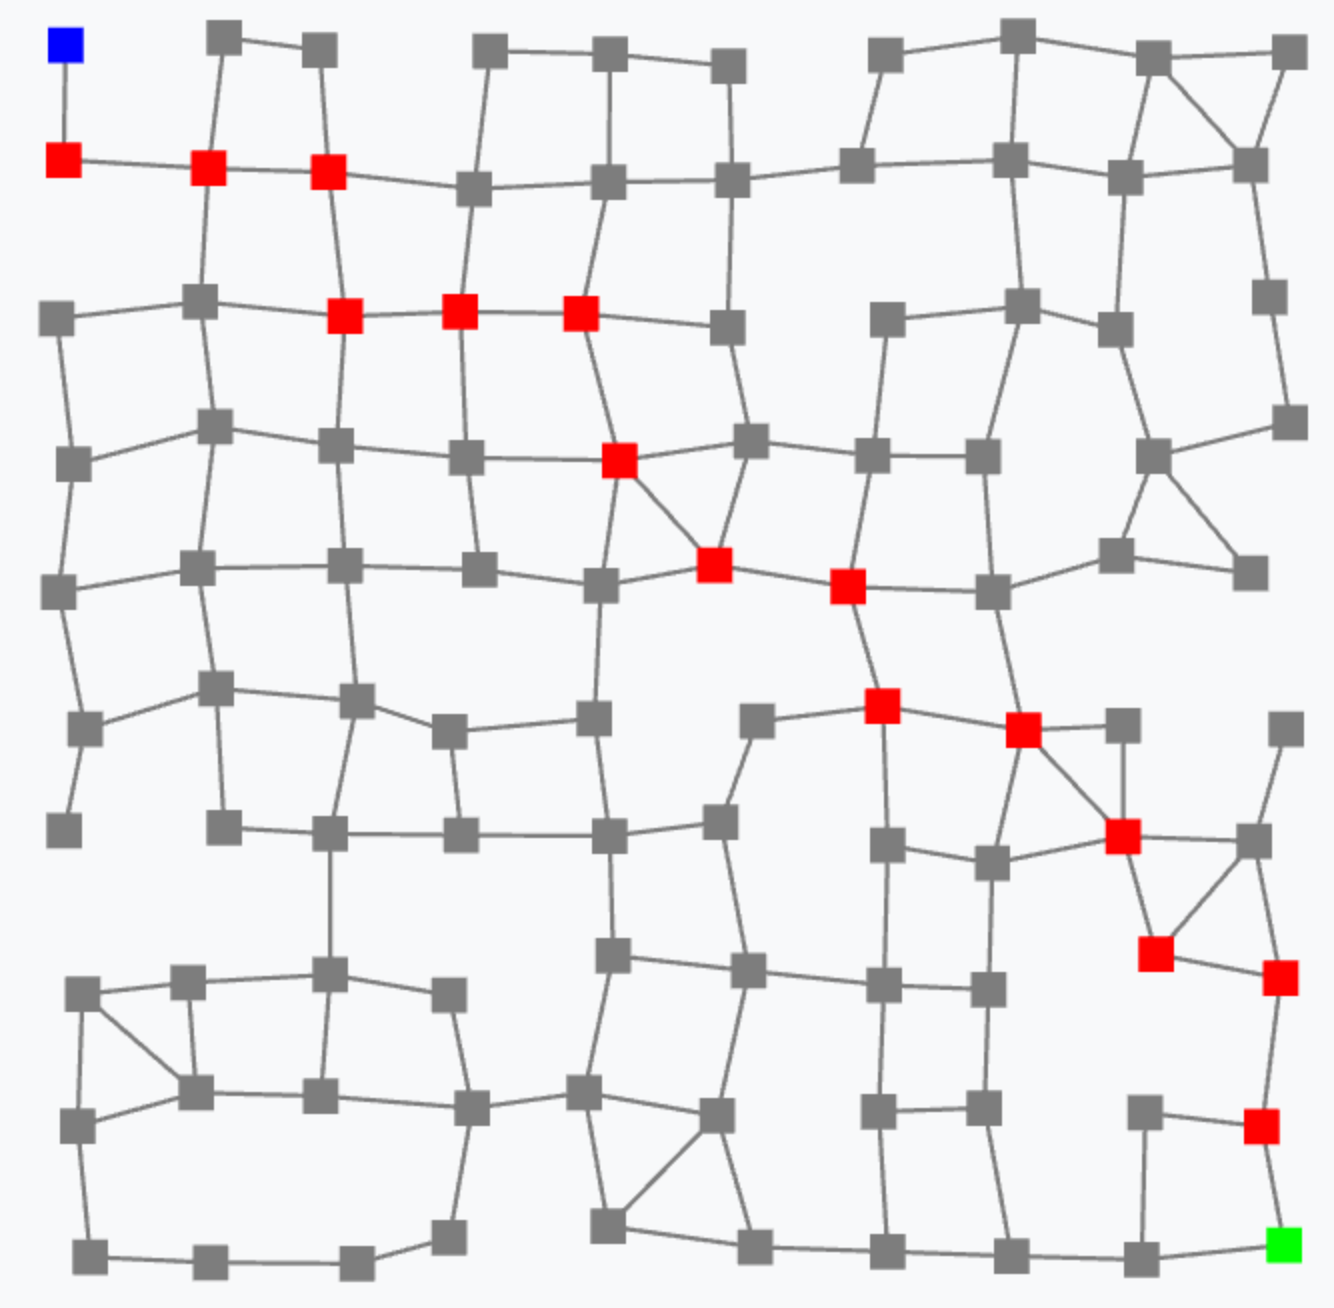
\includegraphics[width=5cm]{img/channel.png}
	\end{column}
\end{columns}
\end{frame}

\begin{frame}{ScalaLoci}
\begin{itemize}
	\item ScalaLoci is a \emph{distributed programming language} embedded into Scala.
 	\begin{itemize}
		\item based on typed-based \emph{multi-tier} programming
  	\item used to describe deployments \& interaction among components
		 \item simplifies developing distributed systems
   	\item reduces error-prone communication code
    \item favors early detection of bugs
	 \end{itemize}
	 \item data are \emph{placed} through distributed data flows, 
	 \item support multiple software architectures (Client Server, P2P, ...) abstracting over low-level communication details and data conversions
	 \item Based on Scala \emph{macro} (< 2.13)
   \item Support several communication protocl (TCP, WebSocket, ...)
   \item Multi-module \& cross-platform 
\end{itemize}
\end{frame}
\begin{frame}[fragile]{ScalaLoci -- Example}
	\begin{alertblock}{}
		\begin{tcolorbox}[left=0pt, top=0pt, bottom=0pt]
			\begin{minted}{scala}
import loci._ // Contexts..
import loci.serializer.upickle._ // Serialization context
import loci.communicator.tcp._ // Communication context
import rescala.default._ // Observable (reactive stream) cotenxt

@multitier object Chat { // a deployment definition
	@peer type Server <: { type Tie <: Multiple[Client] } // pear and connections
	@peer type Client <: { type Tie <: Single[Server] }
	// Message are placed on Deployments
	val message : Evt[String] on Client = on[Client] { Evt[String] }
	// To access to remote data, I must have a Tie
	val publicMessage = on[Server] sbj { client: Remote[Client] =>
		message.asLocalFromAllSeq collect { case (remote, message) if remote == client => message }
	}
	def main() = on[Client] { // Main client logic
		publicMessage.asLocal observe println
		for (line <- scala.io.Source.stdin.getLines) message.fire(line)
	}
}
// Elsewhere...
object Server extends App {
	multitier start new Instance[Chat.Server](listen[Chat.Client] { TCP(43053) })
}
object Client extends App {
	multitier start new Instance[Chat.Client](connect[Chat.Server] { TCP("localhost", 43053) })
}
			\end{minted}
		\end{tcolorbox}
	\end{alertblock}
\end{frame}
%/////////
\frame{\titlepage}
%/////////

%===============================================================================
\section*{\refname}
%===============================================================================

%%%%
\setbeamertemplate{page number in head/foot}{}
%/////////
\begin{frame}[c,noframenumbering, allowframebreaks]{\refname}
%\begin{frame}[t,allowframebreaks,noframenumbering]{\refname}
	\tiny
	\nocite{*}
	\printbibliography
\end{frame}
%/////////

%%%%%%%%%%%%%%%%%%%%%%%%%%%%%%%%%%%%%%%%%%%%%%%%%%%%%%%%%%%%%%%%%%%%%%%%%%%%%%%%
\end{document}
%%%%%%%%%%%%%%%%%%%%%%%%%%%%%%%%%%%%%%%%%%%%%%%%%%%%%%%%%%%%%%%%%%%%%%%%%%%%%%%%
